\documentclass[11pt]{article}
\usepackage[margin=0.75in]{geometry}
\usepackage{setspace}
\usepackage{iftex}
\usepackage{amsmath,amssymb}
\usepackage{graphicx}
\usepackage{enumitem}
\usepackage{pdfpages}
\usepackage{booktabs}
\usepackage{array}
\usepackage{cite}
\usepackage{url}
\usepackage{wrapfig}
\usepackage{float}

\ifPDFTeX
  \usepackage[T1]{fontenc}
  \usepackage{newtxtext,newtxmath}
\else
  \usepackage{fontspec}
  \setmainfont{Times New Roman}
\fi

\setstretch{1.15}
\setlength{\parskip}{0.5em}
\setlength{\parindent}{0pt}
\pagenumbering{arabic}

\begin{document}

% ----------------------------------------------------
% PAGE 1: COVER PAGE
% ----------------------------------------------------

\includepdf[pages=1]{../mb_p3_cover.pdf}

% ----------------------------------------------------
% PAGE 2: MAIN BODY
% ----------------------------------------------------
\section{Focus Area, Rationale, and Stakeholder Relevance}
This project implements a dual extreme ultraviolet (EUV) simulation pipeline to model both the photoabsorption and subsequent core-level Auger electron decay in photoresist materials to evaluate their chemical sensitivity and performance. During EUV lithography, 92 eV exposure first induces photoabsorption to excite or ionize core electrons (e.g., Iodine 4d shell), which subsequently undergo Auger decay cascades. These secondary electrons initiate chemical reactions such as photoacid generation which create patterns in the resists. Understanding both the initial absorption and the subsequent electron emission is essential for optimizing resist sensitivity and resolution at sub-10 nm nodes. The interactive simulation code for our EUV simulation pipeline has been published as a Jupyter notebook~\cite{mb_notebook}.

The primary stakeholders and beneficiaries of this work include:
\begin{itemize}[leftmargin=*,noitemsep,topsep=0pt]
  \item \textbf{Semiconductor Manufacturers and Lithographers:} Guides the predictive design of photoresists to maximize light-absorption and secondary electron yield.
  \item \textbf{Materials Scientists:} Provides a robust computational framework for predicting electron cascade kinetics in halogenated compounds.
\end{itemize}

\section{Technical Methodology and Hybrid Quantum Integration}
Our EUV simulation pipeline is written in PennyLane~\cite{pennylane2018}, and models both photoabsorption and Auger decay:
\begin{enumerate}[leftmargin=*,noitemsep,topsep=0pt]
  \item \textbf{Photoabsorption Spectrum:} Using a time-domain Green's function propagated via a second-order Trotter product formula on a Compressed Double-Factorized (CDF) Hamiltonian, based on~\cite{kharazi2026}.
  \item \textbf{Auger Electron KE Spectrum:} Using a Generative Quantum Eigensolver (GQE)~\cite{gqe2024} combined with the Quantum Self-Consistent Equation-of-Motion (q-sc-EOM) and One-Center Approximation (OCA), based on~\cite{keithley2026}.
\end{enumerate}

\subsection{EUV Photoabsorption Spectrum Simulation}
The EUV photoabsorption channel simulates the dipole-allowed valence-excitation spectrum under 92 eV radiation. We compute the transition dipole moment operators $\hat{m}_\rho$ in the molecular active space and project the ground state wavefunction to obtain initial states $\hat{m}_\rho |I\rangle$ along the Cartesian $x,y,z$ coordinates. We then propagate the states in the time-domain after which measuring the time-dependent expectation values $\langle\hat{m}_\rho(t)\rangle$ yields the time-domain Green's function $G(t)$, which is Fourier-transformed to resolve the absorption spectrum in the frequency domain.

\subsection{EUV Auger Emission: The GQE Challenge and Decay Modeling}
Simulating the Auger emission spectrum requires modeling multi-electron electronic decay from core-ionized and doubly-ionized states. Since the decay transitions are highly sensitive to the ground-state reference, preparing a high-fidelity reference state represents a major GQE challenge. We address this using a hybrid quantum workflow consisting of three stages: GQE, q-sc-EOM and OCA, with an optional classical OpenMolcas RASSI reference.

\subsection{Phase 3 Pipeline Enhancements: Scaling, GPU Acceleration, and Memory Optimization}
In Phase 3, we introduced major architectural and computational enhancements to scale the simulation pipeline from toy molecules ($\rm H_2O$) to realistic halogenated photoresist materials:
\begin{enumerate}[leftmargin=*,noitemsep,topsep=0pt]
  \item \textbf{Target Molecule Scaling to IMePh ($\rm C_7H_7IO$):} We integrated automated 3D geometry querying via PubChem~\cite{pubchem2021} for 4-iodo-2-methylphenol (IMePh), a key EUV photoresist target containing heavy Iodine.
  \item \textbf{Effective Core Potential (ECP) Integration:} To model heavy Iodine without prohibitive qubit counts, we incorporated a \texttt{def2-SVP} small-core ECP that replaces 46 non-participating core electrons while explicitly maintaining the EUV-active 4d shell. Combined with Active Space Selection (AVAS), this reduces the required active space to CAS(16e,\,16o) / 32 qubits.
  \item \textbf{Memory-Efficient Wavefunction Dipole Projection:} We replaced $2^N \times 2^N$ sparse matrix Kronecker products for dipole projections with PySCF's 1-body contraction (\texttt{fci.direct\_spin1.contract\_1e}). Statevector representations are stored as compact sparse dictionaries ($\sim$150~KB) and generated on-demand per Cartesian coordinate, reducing peak host RAM consumption from $>68$~GB down to $<1.5$~GB.
  \item \textbf{GPU Acceleration and Precision Optimization:} We configured PennyLane QNodes to execute on \texttt{lightning.gpu} using CUDA backends. By configuring single-precision \texttt{complex64} statevector representations across all Trotter evolution and q-sc-EOM emission steps, PCIe data transfer overheads were halved and GPU memory bandwidth throughput was doubled.
  \item \textbf{CDF Fragment Truncation:} We implemented compressed double-factorization with fragment truncation, retaining dominant two-body tensor fragments to reduce Trotter gate counts per step by $\sim 70\%$ without loss of physical accuracy.
  \item \textbf{Single-Pass Quantum Evaluation without Snapshots:} For GQE candidate evaluation, we replaced multi-tape \texttt{qml.snapshots} with a direct single-pass \texttt{final\_energy\_circuit} QNode, reducing quantum circuit tape executions per evaluation check by $5\times$.
\end{enumerate}

\section{Data Modeling and Benchmarking Strategy}
Our data modeling strategy utilizes the standard STO-3G basis set. To scale both the photoabsorption and the core-level emission calculations, we incorporate four acceleration techniques:
\begin{enumerate}[leftmargin=*,noitemsep,topsep=0pt]
  \item \textbf{Active Space Selection (AVAS):} Trims molecular orbitals down to active valence electrons and orbitals (e.g., CAS(16e, 16o) / 32 qubits for IMePh) to maintain classical tractability.
  \item \textbf{Effective Core Potential (ECP):} Replaces non-participating core electrons of heavy halogen atoms with pseudopotentials while maintaining core 4d excited state channels.
  \item \textbf{Compressed Double Factorization (CDF):} Compresses the molecular Hamiltonian terms using a Block-Invariant Symmetry Shift (BLISS) and L2-regularized numerical fitting, minimizing the one-norm of the two-body operator.
\end{enumerate}
For validation, our classical benchmarks include exact FCI from PySCF~\cite{pyscf2020} to validate GQE training, and RASSI in OpenMolcas~\cite{openmolcas2020} to validate the Auger spectrum simulation.

\section{Experimental Results and Discussion}
Our results span three molecules of deliberately increasing computational complexity --- from the 2-atom toy system LiH up to the halogenated photoresist IMePh. Each molecule added a new engineering challenge: heavier atoms, larger active spaces, ECP integration, and ultimately the memory wall of q-sc-EOM scaling. Table~\ref{tab:complexity} summarises the pipeline parameters across all three targets.

\begin{table}[H]
\centering
\caption{Molecular complexity progression: qubit counts, active spaces, and CDF compression}
\label{tab:complexity}
\vspace{0.5em}
\begin{tabular}{lccccc}
\toprule
\textbf{Molecule} & \textbf{Qubits} & \textbf{Active Space} & \textbf{CDF Fragments ($L$)} & \textbf{Reduction vs.\ $N^2$} & \textbf{Frobenius Error} \\
\midrule
LiH   & 12 & CAS(4e,\,6o)  & 12 of 36 & 66.7\% & $1.73 \times 10^{-2}$ \\
H$_2$O  & 14 & CAS(10e,\,7o) & 14 of 49 & 71.4\% & $4.10 \times 10^{-2}$ \\
IMePh & 32 & CAS(16e,\,16o) & 10 of 256 & 96.1\% & $1.64 \times 10^{-1}$ \\
\bottomrule
\end{tabular}
\end{table}

\textbf{LiH (12 qubits).}
LiH at CAS(4e,\,6o) is the proof-of-concept benchmark: no heavy atoms, no ECP, and all 12 qubits map directly to the full STO-3G active space. CDF compressed the two-body tensor from an $N^2 = 36$ fragment upper bound down to $L = 12$ retained fragments (66.7\% reduction, Frobenius error $1.73 \times 10^{-2}$). The absorption spectrum resolved light-atom valence excitations and the full dual-channel workflow --- absorption through Auger --- executed end-to-end, validating the pipeline before scaling.

\textbf{H$_2$O (14 qubits).}
H$_2$O at CAS(10e,\,7o) is the most thoroughly validated molecule in our pipeline. CDF compressed $N^2 = 49$ fragments to $L = 14$ (71.4\% reduction, Frobenius error $4.10 \times 10^{-2}$). The \textbf{absorption} spectrum shows good agreement with the CASCI baseline, resolving valence excitations in the 10--45~eV range and confirming no EUV-active dipole transitions near 92~eV in STO-3G---an important negative result that motivates the move to heavier halogenated targets.

For the \textbf{Auger emission} channel, we trained GPTQE and DiTQE for 10{,}000 epochs. GPTQE minimized the H$_2$O ground-state energy to $-74.9650$~Ha (FCI: $-75.0125$~Ha, $\Delta = 0.0475$~Ha). DiTQE initially underperformed due to a causal leakage bug in its multi-headed self-attention block: without a lower-triangular mask, the model could look ahead at future tokens during autoregressive generation. Enforcing causal masking resolved the leak; corrected DiTQE reached $-74.9715$~Ha ($\Delta = 0.0410$~Ha), edging ahead of the GPT baseline. Using these GQE reference states, q-sc-EOM resolved the excited states and OCA yielded Auger decay rates, reproducing the main peak at $E_{\rm kin} = 502.4$~eV in agreement with~\cite{keithley2026} and experimental data~\cite{moddeman1973}.

\textbf{IMePh (32 qubits).}
IMePh ($\rm C_7H_7IO$, 4-iodo-2-methylphenol) is the industrial target: a halogenated EUV photoresist where Iodine 4d core-excitations become active at exactly the 92~eV lithography wavelength. At the STO-3G all-electron level, IMePh demands 148 qubits---completely intractable. A \texttt{def2-SVP} ECP for Iodine reduces this to 146 qubits, and AVAS collapses the chemically active space to CAS(16e,\,16o) / 32 qubits by focusing on the EUV-active 4d shell and adjacent ligand orbitals. CDF compression reaches its highest ratio in our benchmark: truncating to the top $L = 10$ dominant fragments from an $N^2 = 256$ upper bound achieves 96.1\% compression (Frobenius error $1.64 \times 10^{-1}$)---a deliberate lossy truncation that enables fast Trotter gate synthesis at the cost of a slightly elevated Hamiltonian approximation error. We successfully computed the IMePh absorption spectrum and completed GQE training, with only Auger simulation that remains incomplete. Our data shows limitations of such heavy truncation, the absorption spectrum peaks much earlier at around 65 eV.

Figure~\ref{fig:spectra_grid} presents the computed spectra for all three molecules.

\begin{figure}[H]
\centering
\begin{tabular}{>{\centering\arraybackslash}m{0.07\textwidth} >{\centering\arraybackslash}m{0.44\textwidth} >{\centering\arraybackslash}m{0.44\textwidth}}
\toprule
\textbf{Molecule} & \textbf{Photoabsorption Spectrum} & \textbf{Auger Emission Spectrum} \\
\midrule
\textbf{LiH} &
  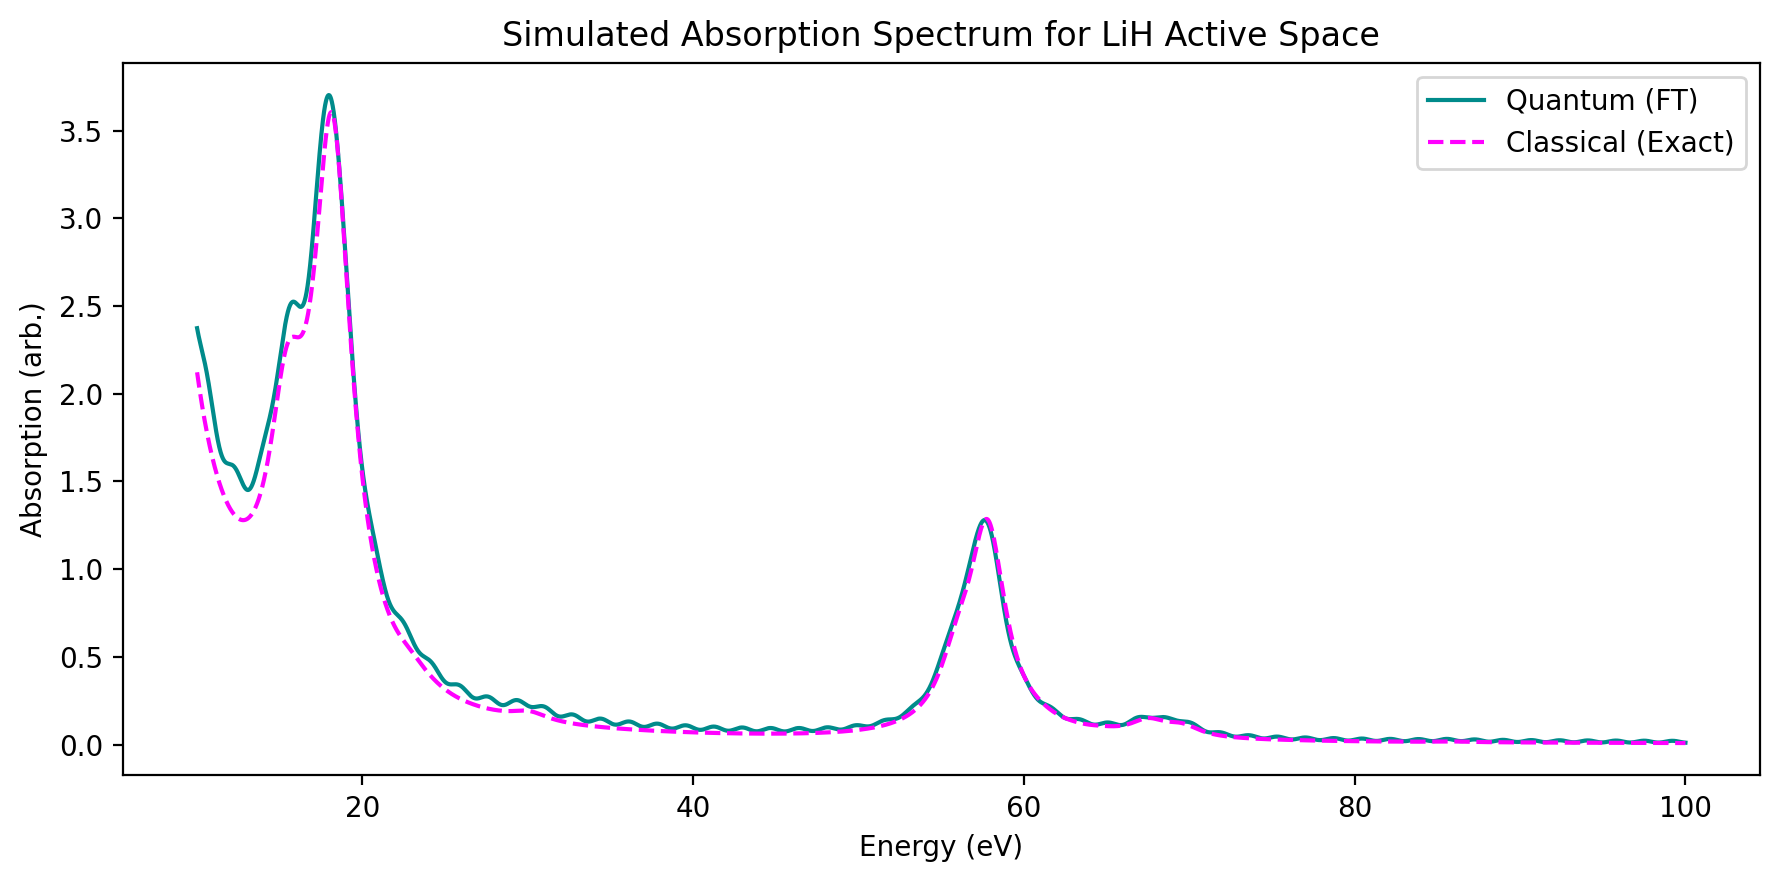
\includegraphics[width=0.44\textwidth, clip]{../../img/lih_abs.png} &
  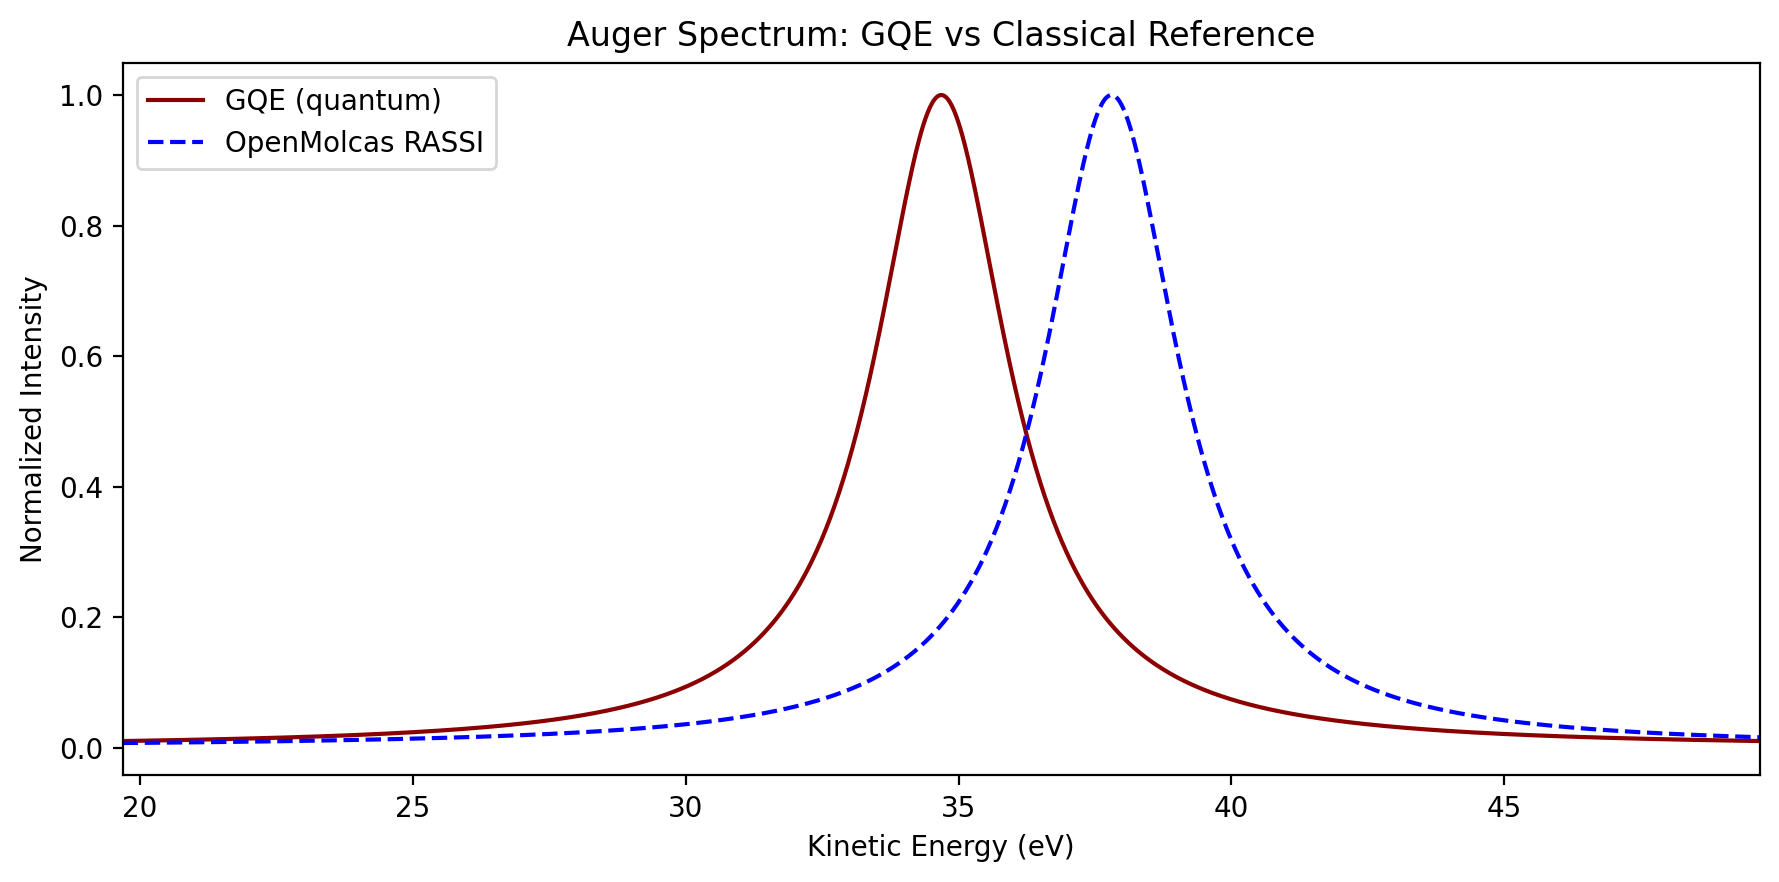
\includegraphics[width=0.44\textwidth, clip]{../../img/lih_ems.png} \\[1ex]
\textbf{H$_2$O} &
  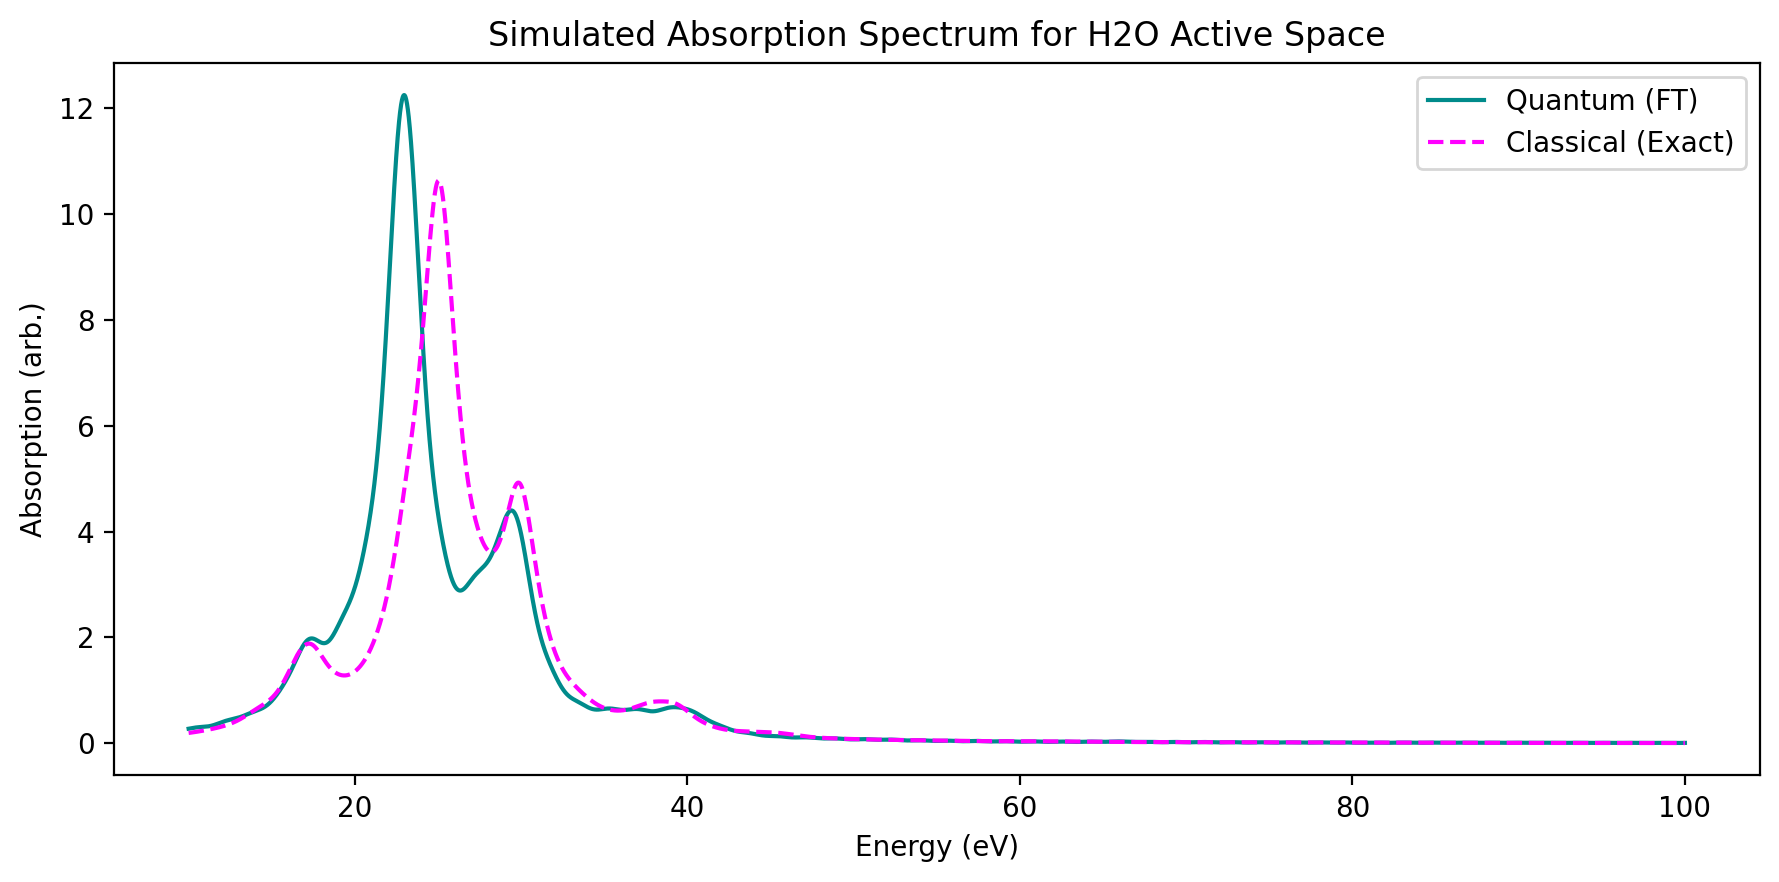
\includegraphics[width=0.44\textwidth, clip]{../../img/h2o_abs.png} &
  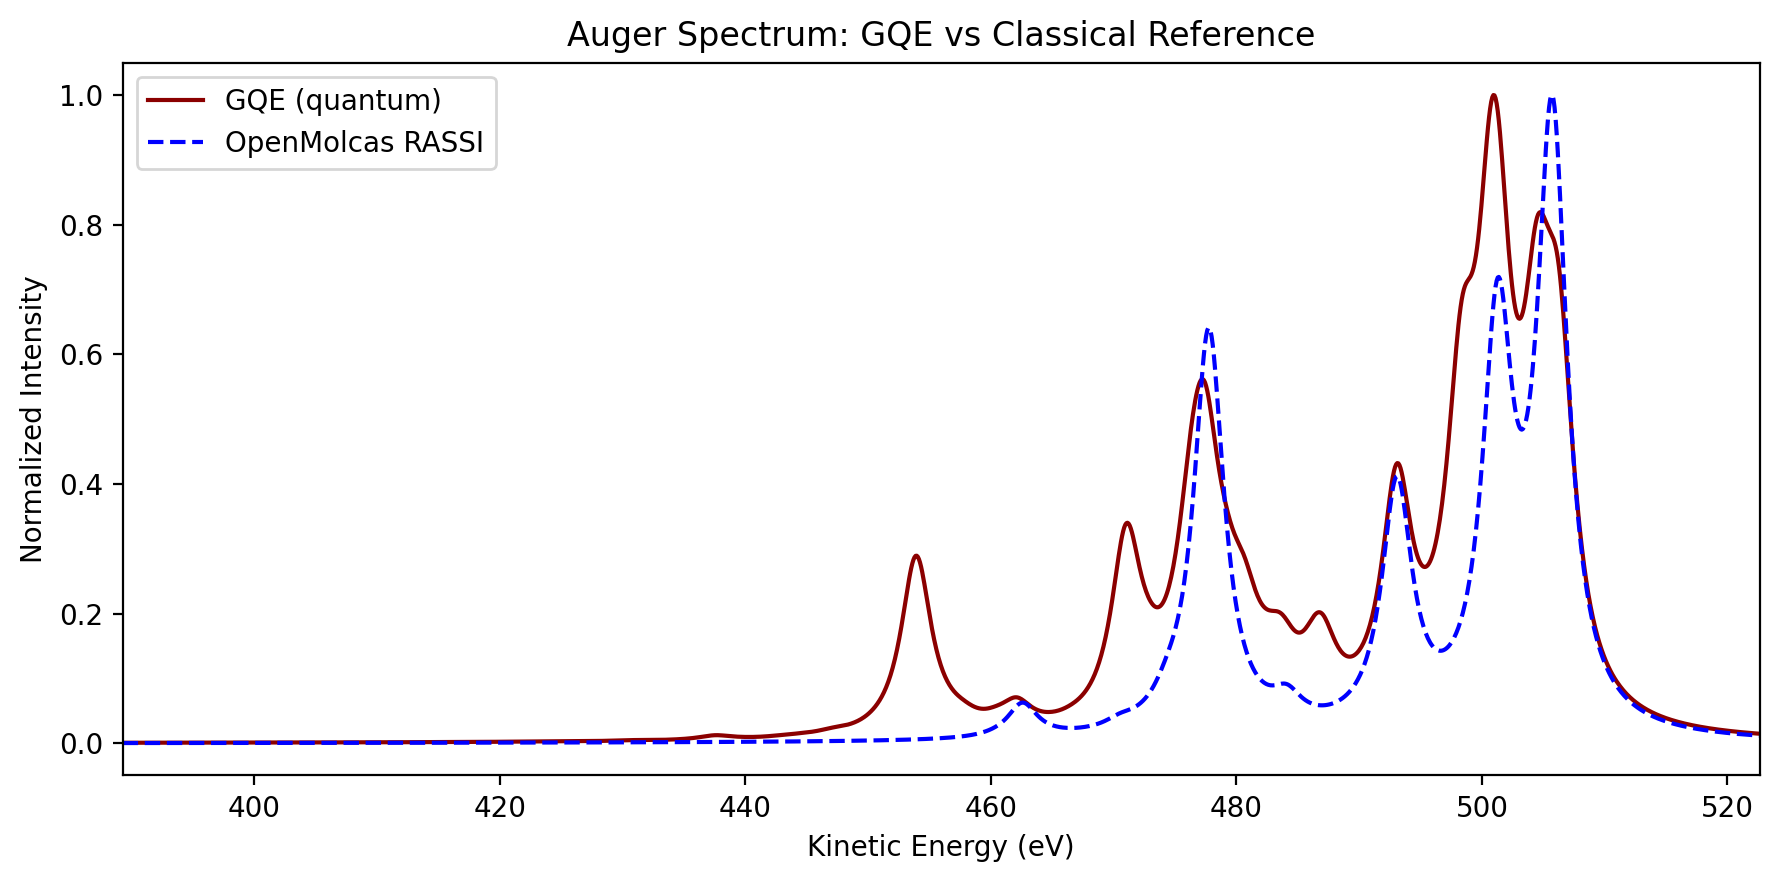
\includegraphics[width=0.44\textwidth, clip]{../../img/h2o_ems.png} \\[1ex]
\textbf{IMePh} &
  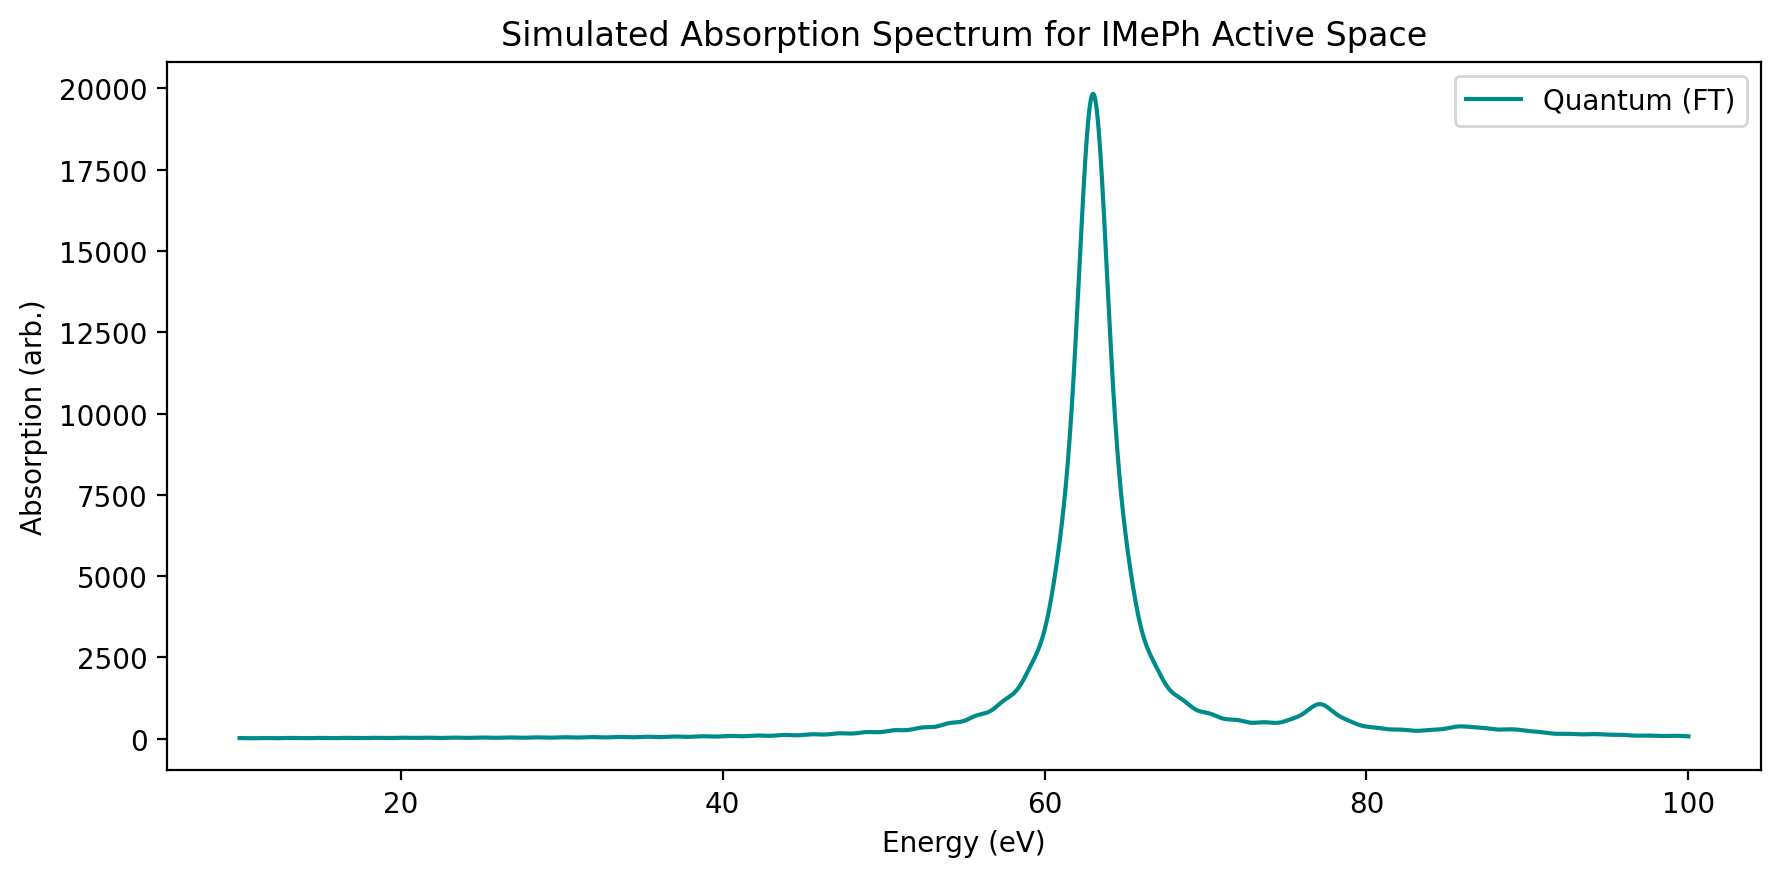
\includegraphics[width=0.44\textwidth, clip]{../../img/imeph_abs.png} &
  \small\textit{Auger spectrum not computed --- q-sc-EOM could not scale to IMePh's $8{,}386$ active-space basis states.} \\[1ex]
\bottomrule
\end{tabular}
\caption{Photoabsorption (left) and Auger electron emission (right) spectra for each target molecule. Absorption spectra are computed via time-domain Trotter evolution on a CDF Hamiltonian. Emission spectra use GQE-prepared reference states with q-sc-EOM and OCA broadened at 1.5~eV. The IMePh Auger emission spectrum is absent as q-sc-EOM could not scale to the $8{,}386$-dimensional active space required at this time.}
\label{fig:spectra_grid}
\end{figure}

\section{Gap Analysis}
\begin{itemize}[leftmargin=*,noitemsep,topsep=0pt]
  \item \textbf{IMePh spectral calculations:} Our primary objective was simulating IMePh spectroscopy. While we successfully captured its absorption spectrum and completed the demanding GQE training, scaling to IMePh's full Auger spectrum proved insurmountable in the given time. Along the way we met many issues like performance bottlenecks, kernel crashes and out of memory errors — many of which were resolved. We have a CPU bound stage in our pipeline that prepares Slater determinants for the two subsequent q-sc-EOM calculations, and we ran out of time and compute due to this unresolved performance bottleneck. We expect that if our H200 instance were left running for another hour or two, it would be able to enter the q-sc-EOM calculation for IMePh.
  \item \textbf{Leveraging CUDA Speedups for Tensor Contraction:} We used GPU acceleration via PyTorch \texttt{einsum}  to rapidly process high-dimensional tensor contractions during OCA. For IMePh, contracting the $8{,}386 \times 28 \times 28$ transition RDM with the 4D continuum-orbital integral tensor ($V_{lmpq}$) is needed to calculate transition amplitudes via Fermi's golden rule. Leveraging fast tensor contractions via cuTENSOR becomes essential for efficient OCA on large molecules. However we were not able to test this acceleration for IMePh, due to the q-sc-EOM dependency.
  \item \textbf{Auger spectral mismatch:} Although close, we were unable to fully reproduce the high spectral agreement with experimental data~\cite{moddeman1973} demonstrated by Keithley et al.~\cite{keithley2026} in their Auger $\rm{H_2O}$ simulations.
  \item \textbf{Qubit tapering:} $\mathbb{Z}_2$ qubit tapering leverages spin parity, particle conservation, and point-group symmetries to reduce the required qubit count by at least 2 qubits for standard molecular Hamiltonians. However, because tapering converts fermionic orbital integrals into entangled Pauli strings, it is structurally incompatible with CDF. Recognizing that circuit execution depth—rather than memory—was our primary bottleneck, we removed qubit tapering from our final pipeline.
  \item \textbf{Block-Invariant Symmetry Shift (BLISS):} We implemented LP-BLISS based on~\cite{lp_bliss}, using linear programming during integral preprocessing to minimize the operator 1-norm. While functional, we omitted BLISS from our final pipeline: BLISS introduces out-of-sector energy shifts that disrupt phase dynamics in time-domain absorption spectroscopy, and time constraints prevented full integration with GQE.
  \item \textbf{Core-Valence Separation (CVS):} We evaluated CVS for preprocessing molecular active spaces, a technique widely used in XAS and XANES spectroscopy to prevent variational collapse. However, integrating CVS into our time-evolution pipeline led to lower accuracy than expected due to artificial decoupling of active interaction blocks.
  \item \textbf{DiffusionGemma:} We wanted to show off this new state-of-the-art open weights diffusion model finetuned on chemistry data and trained to output quantum circuits as our GQE. However diffusion models are notoriously hard to train, so we stuck to GPTnano for final data.
\end{itemize}

\newpage
\bibliographystyle{unsrt}
\bibliography{references}

\end{document}